\documentclass[tikz,border=6pt]{standalone}
\usepackage[T1]{fontenc}
\usepackage{helvet}
\renewcommand{\familydefault}{\sfdefault}
\usepackage{tikz}
\usetikzlibrary{positioning}

\definecolor{ink}{HTML}{1F2937}
\definecolor{muted}{HTML}{6B7280}
\definecolor{head}{HTML}{9A3412}
\definecolor{ssl}{HTML}{C2410C}
\definecolor{sslbg}{HTML}{FFF7ED}

\begin{document}
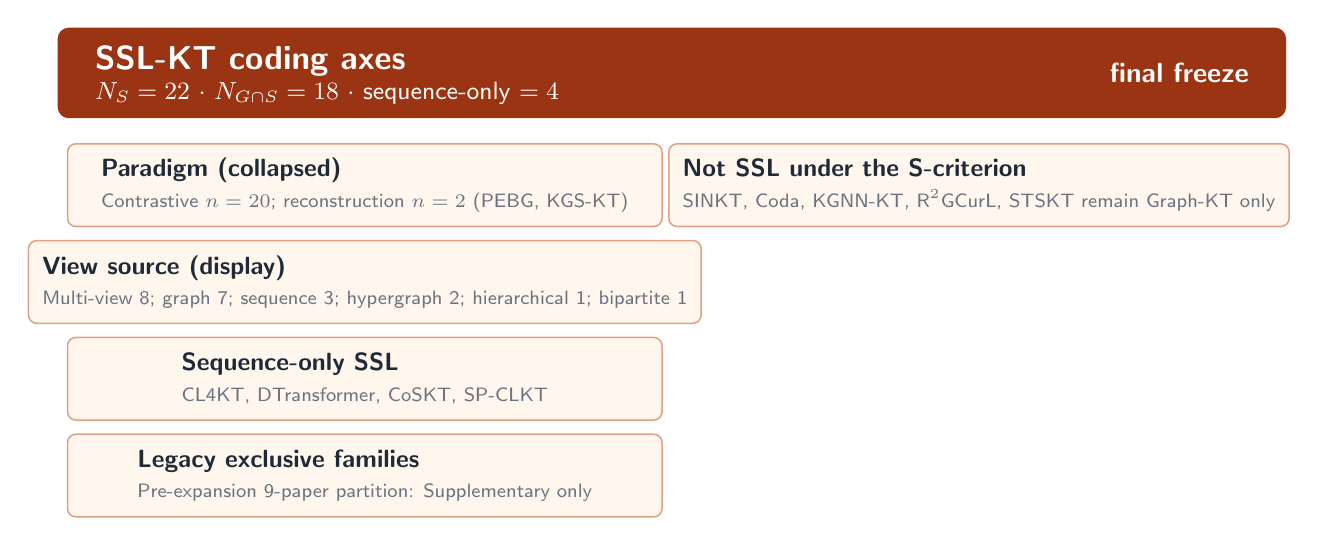
\begin{tikzpicture}[
    font=\sffamily,
    cell/.style={
        rectangle, rounded corners=3pt, align=left,
        minimum width=7.55cm, minimum height=1.05cm,
        inner sep=5pt, draw=ssl!50, fill=sslbg, line width=0.55pt, text=ink
    }
]

\fill[head, rounded corners=4pt] (0,0) rectangle (15.6,1.15);
\node[anchor=west, text=white, font=\sffamily\bfseries\large] at (0.35,0.72)
    {SSL-KT coding axes};
\node[anchor=west, text=white!90, font=\sffamily\small] at (0.35,0.32)
    {$N_S=22$  $\cdot$  $N_{G\cap S}=18$  $\cdot$  sequence-only $=4$};
\node[anchor=east, text=white, font=\sffamily\bfseries] at (15.25,0.58)
    {final freeze};

\node[cell] (a) at (3.90,-0.85) {%
    {\small\bfseries Paradigm (collapsed)}\\[-1pt]
    {\scriptsize\color{muted}Contrastive $n=20$; reconstruction $n=2$ (PEBG, KGS-KT)}};
\node[cell, below=0.16cm of a] (b) {%
    {\small\bfseries View source (display)}\\[-1pt]
    {\scriptsize\color{muted}Multi-view 8; graph 7; sequence 3; hypergraph 2; hierarchical 1; bipartite 1}};
\node[cell, below=0.16cm of b] (c) {%
    {\small\bfseries Sequence-only SSL}\\[-1pt]
    {\scriptsize\color{muted}CL4KT, DTransformer, CoSKT, SP-CLKT}};
\node[cell, below=0.16cm of c] (d) {%
    {\small\bfseries Legacy exclusive families}\\[-1pt]
    {\scriptsize\color{muted}Pre-expansion 9-paper partition: Supplementary only}};

\node[cell] (note) at (11.70,-0.85) {%
    {\small\bfseries Not SSL under the S-criterion}\\[-1pt]
    {\scriptsize\color{muted}SINKT, Coda, KGNN-KT, R$^2$GCurL, STSKT remain Graph-KT only}};

\end{tikzpicture}
\end{document}
